%!TEX root = ../../thesis.tex
%!TEX enableSynctex = true
%*******************************************************************************
%****************************** Third Chapter **********************************
%*******************************************************************************
% **************************** Define Graphics Path **************************
\ifpdf
    \graphicspath{{Chapters/flopt/Figs/Raster/}{Chapters/flopt/Figs/PDF/}{Chapters/flopt/Figs/}}
\else
    \graphicspath{{Chapters/flopt/Figs/Vector/}{Chapters/flopt/Figs/}}
\fi


\makeatletter
\renewcommand*\env@matrix[1][*\c@MaxMatrixCols c]{%
   \hskip -\arraycolsep
   \let\@ifnextchar\new@ifnextchar
   \array{#1}}
\makeatother

\chapter{Frame localisation optical projection tomography}\label{chapter:flopt}

\epigraph{\emph{Pascale Sauvage}}{--- Pablo Vallejo}

In the previous chapters, volumetric imaging was achieved using \gls{wide-field} imaging and a relative scanning motion between the system's focal plane and the sample.
Volumetric imaging can also be achieved by rotating a sample and %reconstructing tomographically.
tomographically reconstructing the \gls{3D} distribution of bright signal (scattering, absorption of luminosity) within the specimen.
%Orthogonal imaging schema can be replaced with pass through imaging provide samples are sufficiently transparent.
%Instead of scanning these samples laterally one can rotate their sample and reconstruct a full three dimensional image.
%As tomographic technology has been shrunk to the millimeter scale, errors induced by hardware become apparent.
Accurate %reconstructions of volumes rely on
tomographic reconstruction relies
heavily on precision movement and rotation.
%This chapter addresses a key downside in traditional approaches to performing full three dimensional reconstructions tomographically.
Here an algorithm will be presented that relies exclusively on multiple (5+) tracked fiducial beads and reconstructs even with systematic mechanical drift.

The projective mathematics introduced in Chapter~\ref{chapter:homography} is a small part of a field of mathematics used in computer vision to to localise (in \gls{3D}) points in space as projected onto multiple view points.
The algorithm presented will use an extension of this projective mathematics to reconstruction \gls{OPT} volumes from each rotational projection.
Considerations were made to combine \gls{OPT} and \gls{light-sheet} imaging within the system constructed in Chapter~\ref{chapter:design}, though this was never realised during this thesis.
\\\\
\emph{It should be noted that, due to conventions within the field of computer vision, all lab frame or \glslink{world point}{world coordinates} will be represented as capital letters (ex.~\gls{X}, \gls{X_c}) in this chapter as in \figurename~\ref{fig:coordinate_system_flopt}.}

% discussed in Chapter \ref{chapter:homography}.%TODO insert chapter.

\pagebreak

\section{Rotational computer tomography in microscopy}

\begin{figure}
    \centering
    \begin{subfigure}[t]{0.475\textwidth}
        \centering
        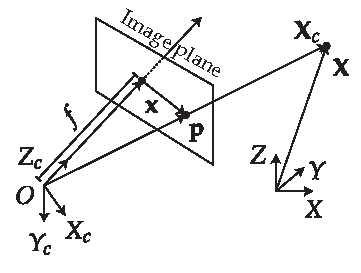
\includegraphics{coordinate_system}
        \caption[Coordinate system]{Coordinate system used in this chapter describing a camera with an associated \gls{image plane} one focal distance \(f\) away, imaging an object at point \(\gls{X}\).
        }
        \label{fig:coordinate_system_flopt}
    \end{subfigure}\hfill
    \begin{subfigure}[t]{0.475\textwidth}
      \centering
      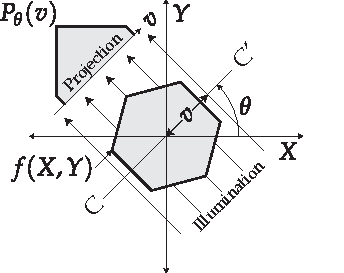
\includegraphics{Chapters/flopt/Figs/PDF/OPT_digram}
      \caption[Principle of OPT]{From an angle \(\theta\), an object \(f(X,Y)\) and the its projection \(P_\theta(t)\) are known.}
      %{Principle of \gls{OPT}, a respective rotation between the sample and the detector illumination pair is iterated.
      % The volumetric image is later reconstructed from the set of detections (1/2D).}
      \label{fig:OPT_digram}
    \end{subfigure}
    \caption[Coordinates and \gls{OPT}]{\gls{X_c} = \((X_c,Y_c,Z_c)\): camera-centered coordinate point in \gls{3D} space.
            \gls{X} = \((X,Y,Z)\): world coordinate point in \gls{3D} space.
            \gls{p} = \((x,y,f)\): ray vector to point of \gls{image plane}.
            \gls{x} = \((x,y)\): \gls{image plane} coordinates.
            \gls{w} = \((u,v)\): pixel coordinates coordinates (not shown).
            The optical axis travels along the\(Z_c\) axis through the \gls{image plane}.}
    % \label{fig:aa}
\end{figure}

%Well establishjed
%Three-dimensional imaging of anatomy in thick biological samples provides valuable data for developmental biology studies.
%Tomographic techniques that generate 3D reconstructions from 2D images such as computed tomography (CT) and magnetic resonance imaging (MRI) are essential in medical applications to visualize morphology in large tissues and organs.
%CT and especially micro-CT can achieve micron-scale resolution using certain contrast agents, however the high doses of radiation used make this unsuitable for repeated experiments on a biological sample.
%Micro-MRI can also achieve resolution in the micron scale, however the cost and size of MRI instruments can be prohibitive for many applications[21].
%Furthermore, neither of these techniques can exploit the plethora of information that can be extracted through fluorescence microscopy.

Sharpe~\emph{et.al} proposed \gls{OPT} in 2002 \cite{sharpe_optical_2002}
using visible light to image transparent or translucent mesoscopic samples, with micro resolution.
\gls{OPT} addresses a scale gap between the photographic techniques (samples larger than 10 mm), and light microscopy techniques (samples smaller than 1 mm) to image biological samples in the \SIrange{1}{10}{\milli\meter} regime.
%Optical Projection Tomography was first proposed by Sharpe in 2002 [30]; it uses visible light to image and create volumetric data of transparent (naturally or artificially) mesoscopic objects (1 - 10 mm) at micron-level resolution.
\gls{OPT} is based on computerised tomography techniques \cite{[17]} in which a set of projections of a specimen are imaged as the specimen travels through a full rotation.
Algorithms exist to then transform this set of images into a
%n $xyz$ image stack.
\gls{3D} image stack in Cartesian \(XYZ\) coordinates.
%A cross-sectional stack of slices from the original object is reconstructed using a back-projection algorithm from the projection images.
\gls{OPT} is non-invasive optically but may require specialist invasive preparation for its samples.
There are two imaging modalities for \gls{OPT}, \gls{eOPT} and \gls{tOPT}.
In \gls{eOPT}, a fluorescent sample is excited using an illumination source off axis to the detection, similar to \gls{light-sheet} but the entire \gls{depth of field} of the detection of objective is illuminated.
% without the excitation being shaped into a sheet.
Scattered illumination photons are rejected at the detector using an appropriate filter.
In tOPT, a white-light source with a diffuser and a collimator is placed along the optical axis to provide near-collimated, uniform illumination onto the sample for transmission to a detector opposite (see \figurename~\ref{fig:OPT_digram}).
Each \gls{photosite} at the detector corresponds to a ray that has passed through the sample and been attenuated by the sample.
The \gls{eOPT} and \gls{tOPT} modes can work in unison to provide contextual information, with the transmission images indicating overall structure (optical density of absorption or scattering) which can be supplemented by the fluorescent signal from a label of interest.
%
% \begin{figure}
%   \centering
%   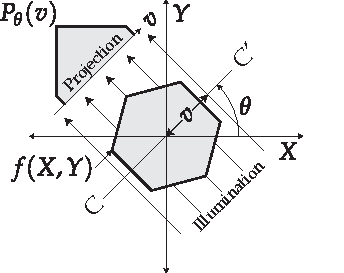
\includegraphics{Chapters/flopt/Figs/PDF/OPT_digram}
%   \caption[Principle of OPT]{Principle of \gls{OPT}, a respective rotation between the sample and the detector illumination pair is iterated.
%   The volumetric image is later reconstructed from the set of detections (1/2D).}
%   \label{fig:OPT_digram}
% \end{figure}

\subsection{Reconstruction}

As the sample is rotated each pixel collects an an intensity \(I(\theta) = I_{n}e^{-k}\) at discrete (\(n\)) angles through a full rotation of the sample; where \(I_{n}\) is the unattenuated radiation intensity from the source to the detector, $k$ is the attenuation caused by the sample along a detected ray an \(I(n)\) is the measured intensity, see \figurename~\ref{fig:OPT_digram}.
Rays from the sample to the detector approximate straight lines, and so the the rays reaching the detector with a line integrals.
A projection is then the resulting intensity profile at the detector for a rotation angle, and the integral transform that results in \(P_\theta(v)\)
%$f(I_i,\theta_n)$
is the \gls{Radon transform}.
% This is defined mathematically as:

\begin{align}
    \intertext{The equation of a set of parallel rays from a source passing through the specimen to a point \(v\) along the detector is:}
    &X\cos(\theta) + Y\sin(\theta) - v = 0 \\
    \intertext{Projecting many such rays through a sample with structure \(f(X,Y)\) gives:}
    P_\theta(v) = &\int_{\infty}^{\infty} \int_{\infty}^{\infty} f(X,Y)\delta (x\cos(\theta)+y \sin(\theta)-v)dX dY
\end{align}

% \begin{figure}
%     \centering
%     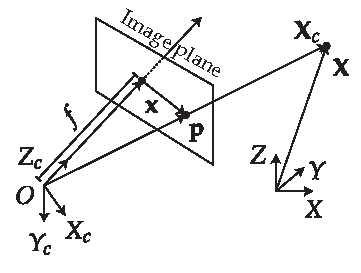
\includegraphics{coordinate_system}
%     \caption{Coordinate system}
%     \label{fig:coordinate_system_flopt}
% \end{figure}

Where $P_\theta(v)$ is the \gls{Radon transform} of $f(X,Y)$ which represents the contrast image of \gls{2D} slice of the specimen.
The \gls{Radon transform} of an image produces a sinugram as in \figurename~\ref{fig:rawinputs}


\begin{figure}
  \centering
  \hfill
  \begin{subfigure}[t]{0.3\textwidth}
    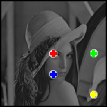
\includegraphics[width=\textwidth]{Chapters/flopt/Figs/PDF/results/no_helix/rawinput_colour}
    \caption{Raw input for OPT simulations, Lena (\(f(x,y)\))}
    \label{fig:raw_input}
  \end{subfigure}\hfill
  \begin{subfigure}[t]{0.3\textwidth}
    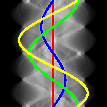
\includegraphics[width=\textwidth]{Chapters/flopt/Figs/PDF/results/no_helix/sinugram_stretch}
    \caption{Image of Lena (\figurename~\ref{fig:raw_input}) after rotation and projection in 2D, giving the sinugram (\(P_{\theta}(v)\)).}
    \label{fig:sinugram_stretch}
  \end{subfigure}
    \hfill
  \label{fig:rawinputs}
  \caption{Reference images for OPT reconstruction.}
  \label{fig:rawinputs}
\end{figure}

% A parallel projection is then just the combination of line integrals $f(I)$ for a constant. % for a constant.

An inverse \gls{Radon transform} is used to recover the original object from the projection data; which is achieved by taking the \gls{Fourier transform} of each projection measurement, then reordering the information from the sample into the respective position in Fourier space.
This is valid due to the Fourier Slice theorem (see Appendix \ref{appendix:fourierslice} for a derivation)\cite{Fourier slice theorem}, %TODO cite
which states that the \gls{Fourier transform} of a parallel projection equivalent to a 2D slice of the Fourier transform original sample.

%A high pass filter such as a ramp filter is commonly used to counter the blurring caused by this oversampling.
% \gls{FBP} can be thought of as smearing the projection data across the image plane, and is expressed in equation form as:

\begin{align}
f_{\text{fpb}}(X,Y) = \int_{0}^{\pi} Q_\theta (X\cos(\theta)+Y\sin(\theta),\theta)dXdY
\end{align}

%\todo{Verify this?!?!?!}
Where $Q_\theta$ is the filtered projection data, and $f_{\text{fpb}}(X,Y)$ is the back-projected image.
A spatial filtering step is applied during back-projection to avoid spatial frequency oversampling during the object’s rotation (see \figurename~\ref{fig:iradon_filter}) %TODO figure 5);
a high pass filter is commonly used to compensate for the perceived blurring.
The blurring arises as \(Q_\theta\) is back-projected (smeared) across the \gls{image plane} for each angle of reconstruction; which means that not only does the back-projection contribute at the line it is intended to (along line \(C\) in \figurename~\ref{fig:coordinate_system_flopt}), but all other points along the back-projecting ray.
% The blurring occurs as \(Q_\theta\) makes the same contribution to the reconstruction for each angle
% will make the same contribution to the reconstruction at all of these points. Therefore, one could say that in the reconstruction process each filtered projection, Qe, is smeared back, or backprojected, over the image plane.

\subsubsection{Aim}

The \gls{Radon transform} relies heavily on the assumption of circular motion with constant angular steps about a vertical axis.
This chapter presents an improved reconstruction method which explains, some of the techniques used in stereoscopic imaging to register back projections rather than relying on line integrals.
The algorithm proposed here is therefore robust to mechanical drifts across acquisitions as well as inconsistent angular steps

\section{Stereoscopic Imaging}

%\subsection{Projective geometry}

%Camera imaging is governed by projective geometry
%Parallel lines project onto a camera will have a vanishing point at the horizon.

%\subsection{Camera projections}

%\todo{Camera projections \ lecture notes 3}

Imaging scenes in stereo allows for the triangulation of individual features in three dimensional space (know as \gls{world point}s) when the features or fiducials in one detector are uniquely identifiable (such as fluorescent beads).

Triangulation requires each feature
% in both images to be the same
to be detected in both images of a stereo imaging system, and for these detections to be correctly associated with one another:
this is known as the correspondence problem.
Many methods exist to ensure that features are %
% known and confidently the same
detected from image data and accurately associated
% image data from
between two cameras or views. %TODO Say more?
Properties of scale independent features and their surrounding pixel environment in one image can be matched to a similar feature in the second image.

Now, suppose we know the relative positions of the two cameras and their intrinsic parameters, such as magnification and pixel offset.
Given the camera parameters, we can translate pixel coordinates \(\gls{w} = (u, v)\) into \gls{image plane} coordinates \(\gls{x}=(x, y)\):
\begin{align}
    u = u_0 + k_u x \\
    v = v_0 + k_v y
\end{align}

Knowing the focal length (\(f\)) of the imaging system, \gls{image plane} coordinates may be translated into a ray in \gls{3D}.
The ray can be defined by a point \gls{p} in camera-centred coordinates, where it crosses the \gls{image plane} as:

\begin{align}
  \mathbf{p} = \begin{bmatrix}
        x\\y\\z
      \end{bmatrix}
\end{align}

From the definition of a \gls{world point}, as observed through an image, we can construct a dual-view model of \gls{world point}s in space as in \figurename~\ref{fig:epi-polar-geom}.
Using a model of a system with two views allows for the triangulation of rays based on image correspondences, this is an important part of stereo-vision.
The most important matching constraint which can be used the \emph{epipolar constraint}, and follows directly from the fact that the rays must intersect in 3D space.
Epipolar constraints facilitate the search for correspondences, they constrain the search to a 1D line in each image.
To derive general epipolar constraints, one should consider the epipolar geometry of two cameras as seen in \figurename~\ref{fig:epi-polar-geom}


The \textbf{baseline} is defined as the line joining the optical centres.
An \textbf{epipole} is the point of intersection of the baseline with the image plan and there are two epipoles per feature, one for each camera.
An \textbf{epipolar line} is a line of intersection of the epipolar plane with an image plane.
It is the image in one camera of the ray from the other camera’s optical centre to the \gls{world point} (\gls{X}).
For different \gls{world point}s, the epipolar plane rotates about the baseline.
All epipolar lines intersect the epipole.

The epipolar line constrains the search for correspondence from a region to a line.
If a point feature is observed at \gls{x} in one image frame, then its location \gls{x'} in the other image frame must lie on the epipolar line.
We can derive an expression for the epipolar line.
The two camera-centered coordinate systems \gls{X_c'} and \gls{X_c} are related by a rotation, \gls{R} and translation, \gls{T} (see in \figurename~\ref{fig:epi-polar-geom}) as follows:

\begin{align}
    \gls{X_c'} &= \gls{R}\gls{X_c'} + \gls{T}  \\
    \intertext{Taking the vector product with \(\gls{T}\), we obtain}
    \gls{T} \times \gls{X_c'} &= \gls{T} \times \gls{R}\gls{X_c}+ \gls{T} \times \gls{T}  \\
    \gls{T} \times \gls{X_c'} &= \gls{T} \times \gls{R}\gls{X_c}\label{eq:Xprime = RTX}
\end{align}

\begin{figure}
  \centering
  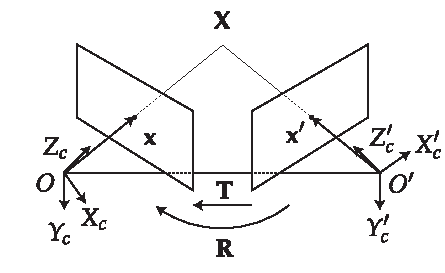
\includegraphics{Chapters/flopt/Figs/PDF/epi-polar-geom}
  \caption{Epi-polar geometry described for two adjacent views (or cameras of a scene). Coordinates as expressed in \figurename~\ref{fig:coordinate_system_flopt} with prime notation (\('\)) denoting the additional right camera view.
  Transforming from right to left camera-centered coordinates (\gls{X_c'} to \gls{X_c}) requires a rotation (\gls{R}) and a translation (\gls{T}).
  }\label{fig:epi-polar-geom}
\end{figure}

\subsection{The Essential matrix}

Taking the scalar product with \gls{X_c'}, we obtain:
\begin{align}
    \gls{X_c'} \cdot (\gls{T} \times \gls{X_c}) &= \gls{X_c'}\cdot (\gls{T} \times \gls{R} \gls{X_c'}) \\
    \gls{X_c'} \cdot (\gls{T} \times \gls{R} \gls{X_c}) &= 0
    \intertext{A vector product can be expressed as a matrix multiplication:}
    \gls{T} \times \gls{X_c} &= \gls{T_times} \gls{X_c}
    \intertext{where}
    \gls{T_times} &=\begin{bmatrix}
    0    & -T_z  & T_y\\
    T_z  & 0     & -T_x\\
    -T_y  & T_x   & 0
    \end{bmatrix}
\end{align}
So equation \eqref{eq:Xprime = RTX} can be rewritten as:

\begin{align}
\gls{X_c'} \cdot (\gls{T_times} \gls{R}\gls{X_c}) = 0 \\
\gls{X_c'} \gls{T} \gls{Essential} \gls{X_c}= 0 \\
\intertext{where}
\gls{Essential} = \gls{T_times} \gls{R}
\end{align}

\gls{Essential} is a $3 \times 3$ matrix known as the \emph{\gls{essential matrix}}.
The constraint also holds for rays \gls{p}, which are parallel to the camera-centered position vectors \gls{X_c}:

\begin{align}
\gls{p'}^T \gls{Essential} \gls{p} = 0 \label{eq:pEp}
\end{align}
This is the epipolar constraint.
If a point \gls{p} is observed in one image, then its position \gls{p'} in the other image must lie on the line defined by Equation~\eqref{eq:pEp}.
The \gls{essential matrix} can convert from pixels on the detector to rays \gls{p} in the world, assuming a calibrated camera (intrinsic properties are known), and pixel coordinates can then be converted to \gls{image plane} coordinates using:
\begin{align}
\begin{bmatrix}
u\\
v\\
1
\end{bmatrix}
&=
\begin{bmatrix}
k_u & 0 & u_0 \\
0 & k_v & v_0 \\
0 & 0 & 1
\end{bmatrix}
\begin{bmatrix}
x\\
y\\
1
\end{bmatrix}
\intertext{We can modify this to derive a relationship between pixel coordinates and rays:}
\begin{bmatrix}
u\\
v\\
1
\end{bmatrix}
&=
\begin{bmatrix}
\frac{k_u}{f} & 0 & \frac{u_0}{f} \\
0 & \frac{k_v}{f} & \frac{v_0}{f} \\
0 & 0 & \frac{1}{f}
\end{bmatrix}
\begin{bmatrix}
x\\
y\\
f
\end{bmatrix}
\intertext{\(\widetilde{\gls{K}}\) is defined as follows:}
\widetilde{\gls{K}} &= \begin{bmatrix}
f k_u & 0 & u_0 \\
0 & f k_v & v_0 \\
0 & 0 & 1
\end{bmatrix}
\intertext{then we can write pixel coordinates in homogenous coordinates:}
\widetilde{\gls{w}} &= \widetilde{\gls{K}} \gls{p}
\end{align}

\subsection{The Fundamental matrix}

\begin{align}
    \intertext{From \eqref{eq:pEp} the epipolar constraint becomes}
    % \mathbf{p'}^T E \mathbf{p} &= 0 \\
    \widetilde{\gls{w'}} ^T \widetilde{\gls{K}}^{-T} E \widetilde{\gls{K}}^{-1} \widetilde{\gls{w}}  &= 0 \\
    \widetilde{\gls{w'}} ^T F \widetilde{\gls{w}}  &= 0
\end{align}
%\subsubsection{Two views}
%\paragraph{Mapping from one camera to another}
%\subsubsection{Three and more views}
The (\(3\times3)\) matrix \gls{F}, is the called the \emph{\gls{fundamental matrix}}.
With intrinsically calibrated cameras, structure can be recovered by triangulation.
First, the two projection matrices are obtained via a \gls{SVD} of the essential matrix.
The \gls{SVD} of the \gls{essential matrix} is given by:

\begin{align}
    \gls{Essential} &= \gls{K'}^T \gls{F} \gls{K} = \gls{T_times} \gls{R} = \mathbf{U}\Lambda \mathbf{V}^T\\%\gls{R} = U\LambdaV^T\\
    \intertext{It can be shown that}
    \hat{\gls{T_times}} &= U \begin{bmatrix}
    0 & 1 & 0 \\
    -1 & 0 & 0 \\
    0 & 0 & 0
    \end{bmatrix} U^T
    \intertext{ and }
    \gls{R} &= U \begin{bmatrix}
    0 & -1 & 0 \\
    1 & 0 & 0 \\
    0 & 0 & 1
    \end{bmatrix} V^T
    \intertext{Then, aligning the left camera and world coordinate systems gives the projection matrices:}
    \mathbf{P} &= \gls{K}    \begin{bmatrix}[c|c]       \mathbf{I} & \mathbf{0}   \end{bmatrix}
    \intertext{ and }
    \mathbf{P}' &= \gls{K'} \begin{bmatrix}[c|c]       \gls{R} & \gls{T}   \end{bmatrix}
\end{align}
Where \( \begin{bmatrix}[c|c] \mathbf{I} & \mathbf{0} \end{bmatrix}\) is the identity matrix augmented column-wise with a zero matrix, and the two projection matrices (\(\mathbf{P}\) and \(\mathbf{P}'\)) project from camera pixel coordinates to world coordinates.
Given these projection matrices, scene structure can be recovered (only up to scale, since only magnitude of \gls{T} (|\gls{T}|) is unknown) using least squares fitting.
Ambiguities in \gls{T} and \gls{R} are resolved by ensuring that visible points lie in front of the two cameras.
As with the \gls{essential matrix}, the \gls{fundamental matrix} can be factorised into a skew-symmetric matrix corresponding
to translation and a 3 x 3 non-singular matrix corresponding to rotation.

\section{The proposed algorithm}

%The rotation may also not be orthogonal to the plane of detection.
The shift of a camera or a camera pair around a scene separated by a transformation matrix (\( \begin{bmatrix}[c|c] \gls{R} & \gls{T} \end{bmatrix}\)) is analogous to a transforming the sample in the fixed view of an imaging detector, as in \gls{OPT}.
During a typical \gls{OPT} acquisition, a marker will appear to follow an elliptical path in the \(XY\) plane.
In the following volume reconstruction there will then be a fitting step to recover the path of the fiducial, to then apply a correction before applying a \gls{Radon transform}.
This type of reconstruction not only ignores any mechanical jitter of the sample but also any affine, systematic, mechanical drift (\(X,Y,Z,\theta,\phi,\psi\)).

We have seen that using two adjacent images, of a scene separated by some rotation and translation, world points in \gls{3D} space may be triangulated within the scene given the rotational and translational matrices of the respect camera views.
The inverse is also possible, given a sufficient number of known fiducial points in a scene the translation and rotation matrices can be recovered.
The recovery of a more exact description of the motion of the scene can eliminate any need for a fitting and may recover and correct for drift, as well as eliminate any mechanical jitter.
Errors may however then be introduced from fiducials mechanically slipping and localisation errors.
Fiducials in this sense refer to an accurately locatable marker common through different views in a sample.

Once a sufficient amount of fidicuials are reliably tracked from the first to the second image, the \glslink{fundamental matrix}{fundamental}, \glslink{essential matrix}{essential} and \Gls{homography} matrices can be computed.
Using the factorisation one of these matrixes, between each adjacent view of a rotating scene, the translation and rotational matrices may be recovered.
Here we will discuss a reconstruction using \gls{F} but the same principle applies for \gls{Essential} and \gls{H}.

\begin{figure}
  \centering
  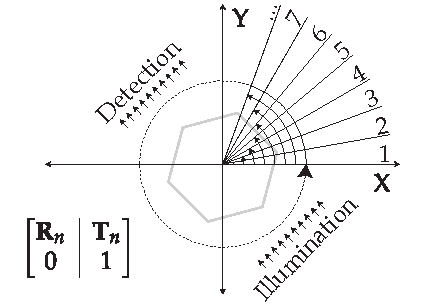
\includegraphics{Chapters/flopt/Figs/PDF/flOPT_principle}
  \caption[Principles of the proposed algorithm]{Principles of the proposed algorithm. Each iteration during an OPT acquisition will have an associate \gls{R} and \gls{T} (shown here in augmented form using homogenous coordinates), these matrices can be recovered from comparing the current iteration (\(n\)) to the next iteration (\(n+1\)).}
\end{figure}

Here are two ways of reconstructing using the \gls{fundamental matrix} as described above.
The first method involves computing \gls{F} for two neighbouring images with 5 or more fiducials, having additional beads helps to remove ambiguity and increase confidence in \gls{F}.
Once \gls{F} is calculated \gls{F} is then decomposed into \(\gls{R}_n\) and \(\gls{T}_n\) between each view \(n\) and \(n+1\).
The image at view \(n+1\) is then back projected along the virtual optical axis within a virtual volume where the sample will be reconstructed.
The size of this back projection and virtual volume is chosen to be suitably large (so that important data is not lost).
Then, all the prior rotation and translation matrices are serially multiplied from \(\begin{bmatrix}[c|c] \gls{R}_0&\gls{T}_0 \end{bmatrix}\) until \(\begin{bmatrix}[c|c] \gls{R}_n&\gls{T}_n \end{bmatrix}\) %$[R_n|T_n]$
, this final matrix is inverted and applied to the back projected volume.
The matrix inversion step is important as it realigns the back projection in the volume to where it originally was compared respective of the first projection.
This process is repeated for every angle and the back projected volume from each step is summed with every other step.
Finally the remaining volume is filtered using a high-pass filter; here a \gls{Ram-Lak filter} is used.
\footnote{Linear real (amplitude) ramp filter in Fourier space}%: \(|v|\)}
By producing a series of transformation matrices from adjacent acquisitions, errors compound and the reconstruction of volumes degrades with more projections, see \figurename~\ref{fig:irandons}.

\begin{figure}
  \centering
  \hfill
  \begin{subfigure}[t]{0.3\textwidth}
    
\includegraphics[width=\textwidth]{Chapters/flopt/Figs/PDF/results/no_helix/iradon_nofilter}
    \caption[Unfiltered iRadon]{Unfiltered output of the \gls{Radon transform} i.e. a reconsutrction}
    \label{fig:iradon_nofilter}
  \end{subfigure}\hfill
  \begin{subfigure}[t]{0.3\textwidth}
    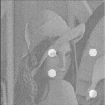
\includegraphics[width=\textwidth]{Chapters/flopt/Figs/PDF/results/no_helix/iradon_filter}
    \caption[Filtered iRadon]{Ram-lak (Fourier ramp) filter applied to \figurename~\ref{fig:iradon_nofilter}.}
    \label{fig:iradon_filter}
  \end{subfigure}
    \hfill
    \label{fig:irandons}
  \caption{The result of a tomographic reconstruction requires Fourier filtering to normalise spatial contrast.}
  \label{fig:irandons}
\end{figure}

The second approach is less prone to compound errors but relies on precise identification and tracking of fiducial markers.
% distinction and tracking fiducials.
Instead of calculating \gls{F} between neighbouring images \gls{F} is calculated between the current projection and the very first projection.
\gls{F} is then decomposed and the transformation matrix is inverted and applied to the back projected volume.
The reoriented back projected volumes are summed and finally filtered to remove the additional spatial frequencies imparted from rotating the sample.

\begin{figure}
    \centering
    \begin{subfigure}[t]{\textwidth}
      \centering
      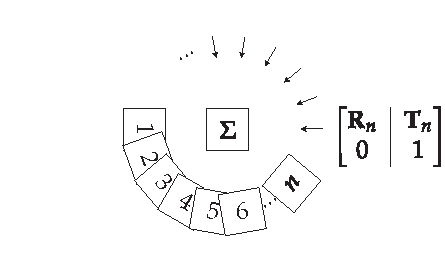
\includegraphics{flopt_algorithm_forward}
      \caption{Forward model}
      \label{fig:flopt_algorithm_forward}
    \end{subfigure}\vspace{0.05\textheight}
    \begin{subfigure}[t]{\textwidth}
      \centering
      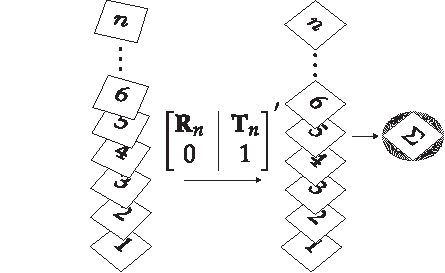
\includegraphics{flopt_algorithm}
      \caption{Reconstruction method, solving the inverse problem.}
      \label{fig:flopt_algorithm_inverse}
    \end{subfigure}
    \caption{
    Two dimensional representation of the reconstruction algorithm.
    (\subref{fig:flopt_algorithm_forward}): For each projection of the object (\(\Sigma\)), at rotation (\(\gls{R}_n\)) and translation (\(\gls{T}_n\)), produces \(n\) data sets.
    (\subref{fig:flopt_algorithm_inverse}): For each data set the rotational and translation matrices are recovered (\(\gls{R}_n'\) and \(\gls{T}_n'\))  and inversely applied to align back project the datasets, the matrices are shown in augmented form using homogenous coordinates.
    The now realigned back projections are summated to produce an unfiltered back projection.
    }
    \label{fig:flopt_algorithm}
\end{figure}

The second approach is robust against compound errors but an additional programatic step is needed to know which beads in the first image correspond to beads in the \(n^{\text{th}}\) image.
This can be is achieved using tracking and momentum particle tracking algorithms, though confounding issues can arise i.e. if a particle orbits too far away or occlusions occur.
In both cases a decomposed \gls{F} matrix will produce four possible transformation pairs (\gls{R},\gls{T}; \gls{R},-\gls{T}; -\gls{R},\gls{T}; -\gls{R},-\gls{T}). %TODO look this up.
Once the transformation matrix between the first view and the second view is calculated the proceeding transformation matrices are then easily chosen by similarity and general direction of motion.
An example of this type of selection would be:
\begin{align}
\min_{I(n)}\left[I(n) = \left(\begin{bmatrix}[c|c] \gls{R}_n&\gls{T}_n \end{bmatrix} - \begin{bmatrix}[c|c] \gls{R}_{n-1}&\gls{T}_{n-1} \end{bmatrix}\right)^2\right]
\end{align}
The first two views are more difficult to choose the correct decomposition for, but it is possible if a suitable ideal matrix is given as a comparison.
Such an ideal matrix is composed using \emph{a priori} knowledge of the likely angle of rotation of the system's imaging properties.

\section{Verification of the proposed algorithm}

To verify that the proposed algorithm successfully reconstructs the specimen%as theorised
, it was applied to simulated data.
The image of Lena
\footnote{Standard reference image data
% The image of Lena is used as a reference to a very early full colour digital scanner.
% The researchers in question realised that their presentation of the scanner's capabilities at a conference lacked a test image.
% The nearest image to hand was a Playboy magazine with Lena Söderberg as the centrefold.
}
is used here as a test image to verify the validity of each reconstruction.
Superimposed on Lena are fiducial beads to track the rotation of the image, see \figurename~\ref{fig:raw_input}.
The reference image was then rotated through \SI{128} angles over $2\pi$ radians and projected along the $Y$ axis and a slice in $XY$ was taken to create a single line projection, shown three dimensionally in \figurename~\ref{fig:recon_iterative}.
This is repeated for each angle with each line projection stacked to create a sinugram, see \figurename~\ref{fig:sinugram_stretch}.

% \begin{figure}
%   \centering
%   \hfill
%   \begin{subfigure}[t]{0.3\textwidth}
%     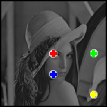
\includegraphics[width=\textwidth]{Chapters/flopt/Figs/PDF/results/no_helix/rawinput_colour}
%     \caption{Raw input for OPT simulations, Lena.}
%     \label{fig:raw_input}
%   \end{subfigure}\hfill
%   \begin{subfigure}[t]{0.3\textwidth}
%     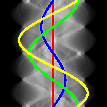
\includegraphics[width=\textwidth]{Chapters/flopt/Figs/PDF/results/no_helix/sinugram_stretch}
%     \caption{Image of Lena (\figurename~\ref{fig:raw_input}) after rotation and projection in 2D, giving the sinugram.}
%     \label{fig:sinugram_stretch}
%   \end{subfigure}
%   \hfill
%   \label{fig:rawinputs}
%   \caption{Reference images for OPT reconstruction.}
% \end{figure}

\begin{figure}
    \begin{subfigure}[t]{\linewidth}
        \centering
        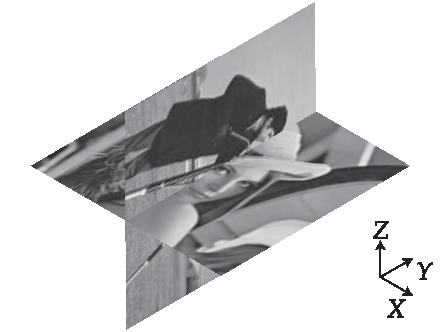
\includegraphics{/ortho_3d_correct}
        \caption{\gls{3D} sample for reconstruction using Cameraman and Lena testcard images.}
        \label{fig:ortho_3d_correct}
    \end{subfigure}
\end{figure}
\begin{figure}
\ContinuedFloat
    \begin{subfigure}[t]{0.2\linewidth}
        \centering
        \includegraphics[width=\textwidth]{/results/3D_python/no_drift/0/xy}\caption{Raw\\Frame (\(n\)): 0\\View: \(XY\)}
    \end{subfigure}\hfill
    \begin{subfigure}[t]{0.2\linewidth}
        \centering
        
\includegraphics[width=\textwidth]{/results/3D_python/no_drift/0/xy_recon}\caption{Reconstructed\\Frame (\(n\)): 0\\View: \(XY\)}
    \end{subfigure}\hfill
    \begin{subfigure}[t]{0.2\linewidth}
        \centering
        \includegraphics[width=\textwidth]{/results/3D_python/no_drift/0/zx}\caption{Raw\\Frame (\(n\)): 0\\View: \(ZY\)}
    \end{subfigure}\hfill
    \begin{subfigure}[t]{0.2\linewidth}
        \centering
        \includegraphics[width=\textwidth]{/results/3D_python/no_drift/0/zx_recon}\caption{Reconstructed\\Frame (\(n\)): 0\\View: \(ZY\)}
    \end{subfigure}
    \begin{subfigure}[t]{0.2\linewidth}
        \centering
        \includegraphics[width=\textwidth]{/results/3D_python/no_drift/1/xy}\caption{Raw\\Frame (\(n\)): 1\\View: \(XY\)}
    \end{subfigure}\hfill
    \begin{subfigure}[t]{0.2\linewidth}
        \centering
        
\includegraphics[width=\textwidth]{/results/3D_python/no_drift/1/xy_recon}\caption{Reconstructed\\Frame (\(n\)): 1\\View: \(XY\)}
    \end{subfigure}\hfill
    \begin{subfigure}[t]{0.2\linewidth}
        \centering
        \includegraphics[width=\textwidth]{/results/3D_python/no_drift/1/zx}\caption{Raw\\Frame (\(n\)): 1\\View: \(ZY\)}
    \end{subfigure}\hfill
    \begin{subfigure}[t]{0.2\linewidth}
        \centering
        \includegraphics[width=\textwidth]{/results/3D_python/no_drift/1/zx_recon}\caption{Reconstructed\\Frame (\(n\)): 1\\View:\(ZY\)}
    \end{subfigure}
    \begin{subfigure}[t]{0.2\linewidth}
        \centering
        \includegraphics[width=\textwidth]{/results/3D_python/no_drift/dots/xy}%\caption{Raw data. Frame (\(n\)): , View: \(xy\)}
    \end{subfigure}\hfill
    \begin{subfigure}[t]{0.2\linewidth}
        \centering
        
\includegraphics[width=\textwidth]{/results/3D_python/no_drift/dots/xy_recon}%\caption{Reconstructed\\Frame (\(n\)):0, View:\(xy\)}
    \end{subfigure}\hfill
    \begin{subfigure}[t]{0.2\linewidth}
        \centering
        \includegraphics[width=\textwidth]{/results/3D_python/no_drift/dots/zx}%\caption{Raw data. Frame (\(n\)): , View: \(zy\)}
    \end{subfigure}\hfill
    \begin{subfigure}[t]{0.2\linewidth}
        \centering
        \includegraphics[width=\textwidth]{/results/3D_python/no_drift/dots/zx}%\caption{Reconstructed\\Frame (\(n\)):, View:\(zx\)}
    \end{subfigure}
    \begin{subfigure}[t]{0.2\linewidth}
        \centering
        \includegraphics[width=\textwidth]{/results/3D_python/no_drift/31/xy}\caption{Raw\\Frame (\(n\)): 31\\View: \(XY\)}
    \end{subfigure}\hfill
    \begin{subfigure}[t]{0.2\linewidth}
        \centering
        
\includegraphics[width=\textwidth]{/results/3D_python/no_drift/31/xy_recon}\caption{Reconstructed\\Frame (\(n\)): 31\\View: \(XY\)}
    \end{subfigure}\hfill
    \begin{subfigure}[t]{0.2\linewidth}
        \centering
        \includegraphics[width=\textwidth]{/results/3D_python/no_drift/31/zx}\caption{Raw\\Frame (\(n\)): 31\\View: \(ZY\)}
    \end{subfigure}\hfill
    \begin{subfigure}[t]{0.2\linewidth}
        \centering
        \includegraphics[width=\textwidth]{/results/3D_python/no_drift/31/zx_recon}\caption{Reconstructed\\Frame (\(n\)): 31\\View: \(ZY\)}
    \end{subfigure}
    \caption{a \gls{3D} test-volume of two orthogonal and different testcard images was used to verify the reconstructive capabilities of the proposed algorithm.
    The results are unfiltered for clarity of demonstrating the iterative reconstruction.}
    \label{fig:recon_iterative}
\end{figure}

\begin{figure}
  \centering
  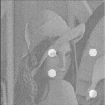
\includegraphics[width=0.3\textwidth]{Chapters/flopt/Figs/PDF/results/no_helix/flopt_filter}
\caption{Filtered reconstruction of a reference image using the new proposed algorithm, (\(XY\))}
\label{fig:flopt_filter}
\end{figure}

In the standard approach for \gls{OPT} reconstruction, the \gls{sinugram} undergoes the inverse \gls{Radon transform}, see \figurename~\ref{fig:iradon_nofilter} and then post-filtering, see \figurename~\ref{fig:iradon_filter}.
This step is substituted for the proposed algorithm; in \figurename~\ref{fig:flopt_comparison_line_profile} the two techniques are compared for ideal conditions of smooth, predictable rotation.
The proposed algorithm produces %(see )
a faithful reconstruction on the original image, as shown in \figurename~\ref{fig:flopt_filter} %with some minor deviations.
Both techniques lose some of the original contrast of the object due to under-sampling of rotations.
When taking the histogram of the absolute pixel-wise difference between the original source image to the images produced by the new algorithm and the \gls{Radon transform},
% there is good overlap between the two,
see \figurename~\ref{fig:flopt_histogram}.
The mean square errors (\gls{MSE}, see Equation~\eqref{eq:mse}) of the new algorithm and the \gls{Radon transform} are \SI{15.01}\% and 14.84\% respectively, see \figurename~\ref{fig:flopt_histogram} for a histogram of a pixel-wise comparison.
This suggests that the new algorithm is producing an accurate reconstruction of the object, similar to the standard \gls{Radon transform}.
%, see \figurename~\ref{fig:flopt_histogram}

\begin{align}
    \operatorname{\gls{MSE}}=\frac{1}{n}\sum_{i=1}^n(Y_i-\hat{Y_i})^2 \label{eq:mse} % \intertext{Where \(\hat{Y_i}\) is the ith value and Y_i }
\end{align}

\begin{figure}
  \centering
  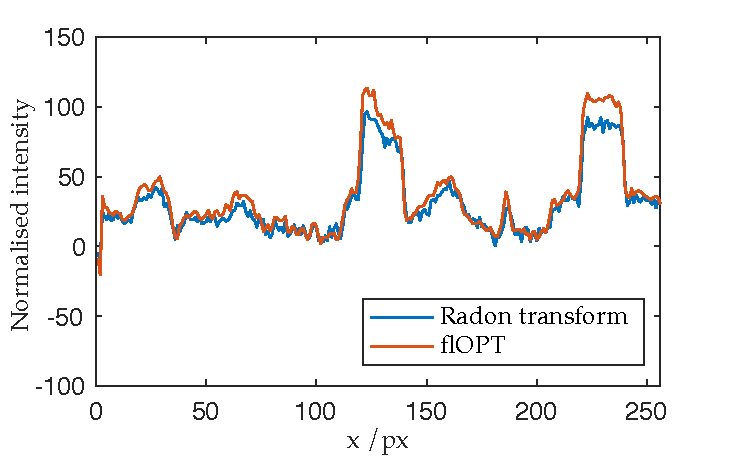
\includegraphics{Chapters/flopt/Figs/PDF/results/comparison_line_profile}
  \caption{Line profile comparison of the reconstruction of a reference image computationally rotated, projected and reconstructed using the standard \gls{Radon transform} and the new proposed algorithm.}
  \label{fig:flopt_comparison_line_profile}
\end{figure}

\begin{figure}
  \centering
  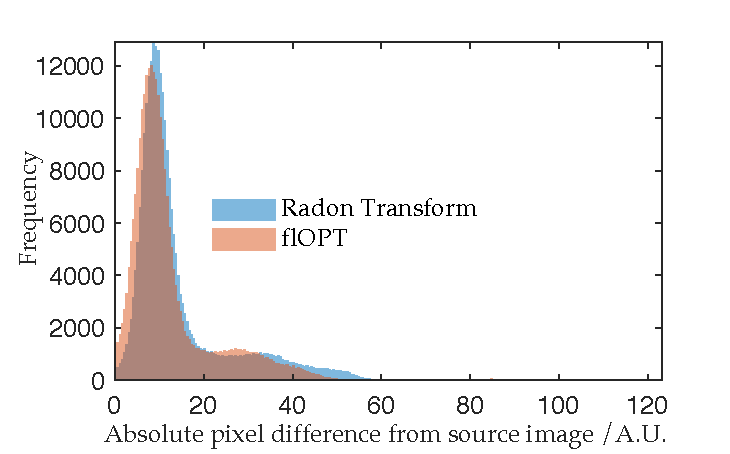
\includegraphics{Chapters/flopt/Figs/PDF/results/flopt_histogram}
  \caption{Histogram of of pixel values compared between reconstructions using flOPT and the \gls{Radon transform}.
  The shift of the histogram to towards overall lower deviance from the source image suggests the flOPT algorithm out performs the \gls{Radon transform}}
  \label{fig:flopt_histogram}
\end{figure}

%However, the proposed algorithm fairs worse in terms of contrast compared to a \gls{Radon transform}.

The more challenging case of a sample drifting, with a constant velocity, systematically along the \(X\) axis was then considered; this produced a helical path of a single fiducial within the sample, see \figurename~\ref{fig:flopt_helix_sinugram}.
In \figurename~\ref{fig:unfilttered_reconstruction_helix_iradon}, the \gls{Radon transform} entirely fails to produce a recognisable reproduction of the test image with the addition of a slight helicity to the rotation.
The proposed algorithm produces an equivalent result to that of a sample rotating without any systematic drift, see \figurename~\ref{fig:iradon_filter}.
In \figurename~\ref{fig:helical_comparison} the respective images from each algorithm were compared, as before, while the helical shift was incremented.
See \figurename~\ref{fig:flopt_helix_sinugram} for a \gls{sinugram} of a sample whereby a helical shift has been induced.
When using correlation as a metric of reproduction quality, at zero helicity, the new algorithm fairs slightly worse at 94\% correlation compared to the \gls{Radon transform} at 96\%.
As expected, the \gls{Radon transform} rapidly deteriorates once a systematic drift is applied; where-as the new algorithm maintains quality of reconstruction, see \figurename~\ref{fig:helical_comparison}.

\begin{figure}
  \centering
  \hfill
  \begin{subfigure}[t]{0.3\textwidth}
    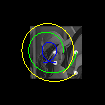
\includegraphics[width=\textwidth]{Chapters/flopt/Figs/PDF/results/helix/topdown_bead_paths}
    \caption{Top down views ($XY$) of the source image with the fiducial paths marked.}
    \label{fig:topdown_bead_paths}
  \end{subfigure}\hfill
  \begin{subfigure}[t]{0.3\textwidth}
    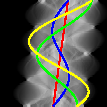
\includegraphics[width=\textwidth]{Chapters/flopt/Figs/PDF/results/helix/sinugram_stretch}
    \caption{Sinugram ($XN$) of a sample whose axis of rotation has a systematic drift}
    \label{fig:flopt_helix_sinugram}
  \end{subfigure}
    \hfill
    \label{fig:flopts}
  \caption{Comparison of the two reconstructions under sample imaging with a systematic drift, in 3D though represented here in 2D.}
\end{figure}
\begin{figure}
  \centering
  \hfill
  \begin{subfigure}[t]{0.3\textwidth}
    
\includegraphics[width=\textwidth]{Chapters/flopt/Figs/PDF/results/helix/unfilttered_reconstruction_helix_iradon}
    \caption{Unfiltered reconstruction using a \gls{Radon transform}, (\(XY\))}
    \label{fig:unfilttered_reconstruction_helix_iradon}
  \end{subfigure}\hfill
  \begin{subfigure}[t]{0.3\textwidth}
    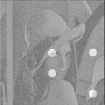
\includegraphics[width=\textwidth]{Chapters/flopt/Figs/PDF/results/helix/filtered_recon_helix}
    \caption{Filtered reconstruction using the new algorithm, (\(XY\))}
    \label{fig:filtered_recon_helix}
  \end{subfigure}
    \hfill
    \label{fig:flopts}
  \caption{Comparison of the two reconstructions under sample imaging with a systematic drift, in 3D though represented here in 2D.}
\end{figure}
\begin{figure}
  \centering
  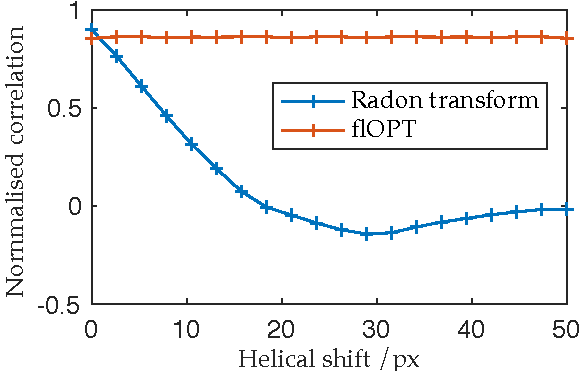
\includegraphics{Chapters/flopt/Figs/PDF/results/correlation_helicity}
  \caption{2D correlation of the source image shows that flOPT does not degrade under systematic drift compared to \gls{Radon transform}s.}
  \label{fig:helical_comparison}
\end{figure}

\subsection{Recovery of R and T using matrix decomposition}

To quantitatively verify that the matrix decomposition technique was valid and robust, the accuracy of the reproduction of \gls{R} and \gls{T} was tested directly.
The original \gls{R} and \gls{T} matrices were computed and compared to \gls{R} and \gls{T} generated from matrix decomposition, this absolute difference was computed element-wise in each matrix and then an average for each matrix was taken.
Overall the worst case scenario produced a percentage error of \SI{2}{\percent} see \figurename~\ref{fig:pc_sum_decompose} for full statistics.
The accuracy of the calculated \gls{R} and \gls{T} did deteriorate when adding in additional degrees of combined movement, but with no correlation between the degree of helicity and the error produced.
% but the severity of this movement appeared to no trending effect.
Consistently the translational matrix (\gls{T}) was more accurately reproduced, this is likely due to there being fewer of degrees of freedom for errors to spread over.

%The images produced are a more faithful reproduction of the source image as the degree of helicity is increased.
%This effect may be due to the additional sampling induced by adding another degree of movement, that is the systematic drift.

%Textwidth is \the\textwidth


\begin{figure}
  \centering
    \begin{subfigure}[t]{0.5\textwidth}
      \captionsetup{width=0.8\textwidth}
      \centering
      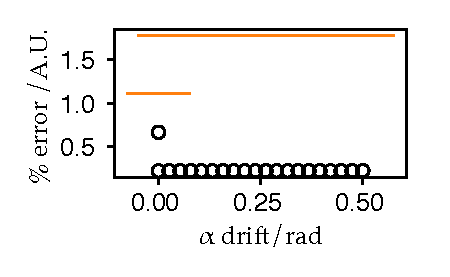
\includegraphics{Chapters/flopt/Figs/PDF/results/helix/decompose/pc_sum_rot_alpha}
      \caption{Rotation matrix, with angular drift in $\alpha$}\label{fig:pc_sum_rot_alpha}
    \end{subfigure}\hfill
    \begin{subfigure}[t]{0.5\textwidth}
      \captionsetup{width=0.8\textwidth}
      \centering
      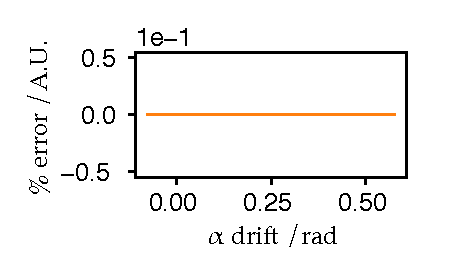
\includegraphics{Chapters/flopt/Figs/PDF/results/helix/decompose/pc_sum_trans_alpha}
      \caption{Translation matrix, with angular drift in $\alpha$}\label{fig:pc_sum_trans_alpha}
    \end{subfigure}
    \bigskip
        \begin{subfigure}[t]{0.5\textwidth}
          \captionsetup{width=0.8\textwidth}
          \centering
          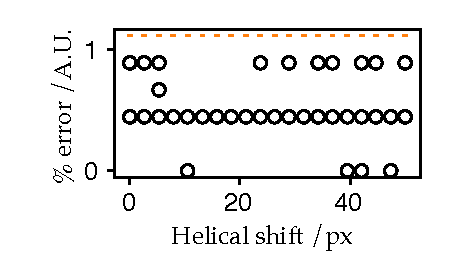
\includegraphics{Chapters/flopt/Figs/PDF/results/helix/decompose/pc_sum_rot_tx}
          \caption{Rotation matrix, with helical drift in $x$ only}\label{fig:pc_sum_rot_tx}
        \end{subfigure}\hfill
        \begin{subfigure}[t]{0.5\textwidth}
          \captionsetup{width=0.8\textwidth}
          \centering
          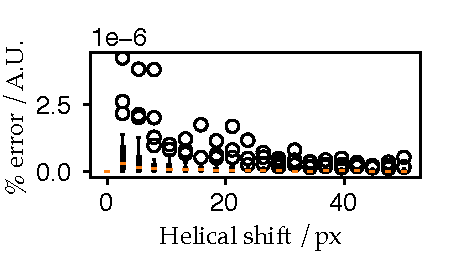
\includegraphics{Chapters/flopt/Figs/PDF/results/helix/decompose/pc_sum_trans_tx}
          \caption{Translation matrix, with helical drift in $x$ only} \label{fig:pc_sum_trans_tx}
        \end{subfigure}
    \bigskip
        \begin{subfigure}[t]{0.5\textwidth}
          \captionsetup{width=0.8\textwidth}
          \centering
          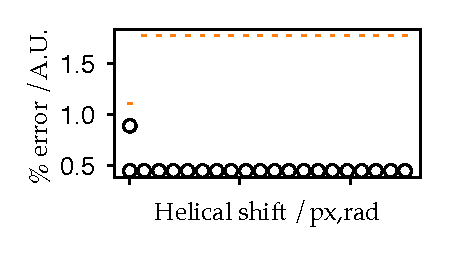
\includegraphics{Chapters/flopt/Figs/PDF/results/helix/decompose/pc_sum_rot_both}
          \caption{Rotation matrix, with angular drift in $\alpha$ and helical drift in $x$}\label{fig:pc_sum_rot_both}
        \end{subfigure}\hfill
        \begin{subfigure}[t]{0.5\textwidth}
          \captionsetup{width=0.8\textwidth}
          \centering
          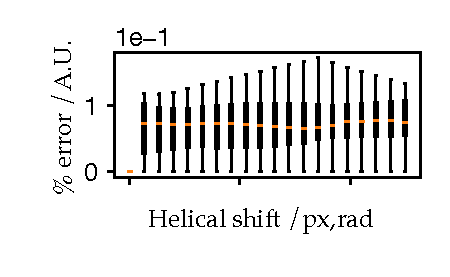
\includegraphics{Chapters/flopt/Figs/PDF/results/helix/decompose/pc_sum_trans_both}
          \caption{Translation matrix, with angular drift in $\alpha$ and helical drift in \(X\)}\label{fig:pc_sum_trans_both}
        \end{subfigure}
          \caption{Box plots demonstrating that the rotational and translations matrices can be recovered accurately from fiducial marker positions.
          Panels \ref{fig:pc_sum_rot_alpha} and \ref{fig:pc_sum_trans_alpha} introduce an angular drift during rotation, to an observer at the detector this would appear as a tip of the sample towards them, causing precession.
          Panels \ref{fig:pc_sum_rot_tx} and \ref{fig:pc_sum_trans_tx} introduce a lateral drift in \(X\) causing a helical path to be drawn out.
          Panels \ref{fig:pc_sum_rot_both} and \ref{fig:pc_sum_trans_both} combine the two effects.
          In all cases the percentage error introduced by the the addition of undesirable additional movements was on the order of $<2\%$.
          }
          \label{fig:pc_sum_decompose}
\end{figure}

\section{Discussion}

A new algorithm for reconstructing OPT data has been demonstrated.
The new algorithm uses multiple fiducials to recover the matrix which describes the rotation and translation of the sample.
The quality of the reconstructions when compared to a standard \gls{Radon transform} shows a slight improvement, with a great effect when a systematic drift is introduced.
The measure the accuracy of the decomposition of \gls{F} into \gls{R} and \gls{T} they were compared to the ground truth matrices.
The element-wise absolute difference \(\left(\frac{x-y}{2(x+y)}\right)\) of each matrix was averaged across the matrix for \gls{R} and \gls{T}.
In the worst case scenario a maximum of \SI{2}{\percent} average absolute difference was found between ground truth and recovered matrices,
% When comparing the
% expected matrices to the recovered matrices a
% ground truth matrices to the recovered matrices were compared using the average of the element-wise using square differences
% peak of \SI{2}{\percent} difference is found between the two when considering worst case scenarios;
suggesting the technique is robust to all forms of drift and general instability.
Such an algorithm could be used to help in minimising ghosting effects seen in real samples; particularly in samples where slipping is likely to occur such as in gels or in cheaper \gls{OPT} systems which tend to be more mechanically unstable and imprecise.

\section{Future work}

\subsection{Bead Tracking}
The work presented here is, so far, is a proof-of-concept demonstrated by simulation and reconstruction from ground-truth testcard objectives, and requires several further steps in order apply it to real \gls{OPT} data.
Firstly, a bead-tracking algorithm\cite{crockerMethodsDigitalVideo1996a} will need to be created to track multiple beads concurrently in an image series.
A sensible approach would be to have a user select the fiducials in the image on the first frame and template match in a small window around the selection; this is similar to the algorithm described in Chapter \ref{chapter:spt}. %TODO insert chapter
Template matching is robust to occlusions provided the fidcuial is not fully eclipsed.
If two fiducials occlude each other however, this algorithm may switch their identities or both tracking windows may follow one bead.
This is a common problem in particle tracking algorithms, but is solved by using a weighted likelihood based on momentum\cite{chenouardMultipleHypothesisTracking2013}.

The likelihood of a bead occlusion occurring will increase with he introduction of additional beads into the sample.
As such occluded beads may need to be omitted.% and possibly interpolated for.
Egregious outliers may be found by tracking a \emph{confidence} estimator as the bead rotates as in
% A primitive estimator would be the pixel-wise sum of intensities in the result of a correlative template matching.
% Whilst this confidence value itself has no physical interpretation, any stark changes in the derivative will be suggestive of an occlusion or mis-tracking of some variety, see
\figurename~\ref{fig:confidence_bead_tracking}.

\begin{figure}
  \centering
  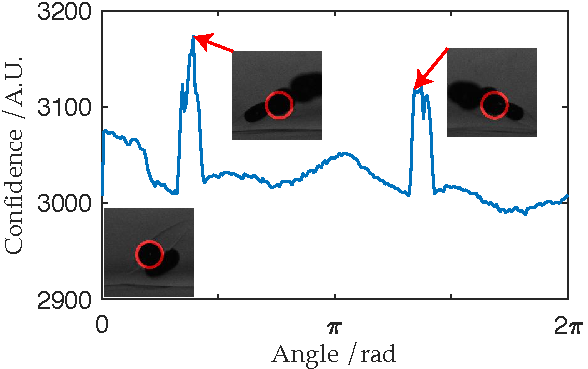
\includegraphics{Chapters/flopt/Figs/PDF/results/confidence_bead_tracking}
  \caption{A plot of the confidence value of a single fiducial bead being tracking \emph{in vivo}.
  Sharp changes in the confidence value occur when the fiducial bead is occluded.
  The image at the origin shows the fiducial being tracked well in the first frame.
  (Images courtesy of Pedro Vallejo)
  }
  \label{fig:confidence_bead_tracking}
\end{figure}

\subsection{Multiple views tracking}
The theory backing the proposed algorithm relies on triangulation between two view points.
In this work the two view points refer to the image at frames \(n\) and \(n+1\).
However, it is possible to use three separate views (frames \(n\), \(n+1\) and \(n+2\)) to reconstruct a scene, one such approach being quaternion tensors.
Working with tensors is computationally and mathematically more challenging, but a future iteration of the algorithm presented here may benefit from using three views to provide a more accurate transformation matrix.
Beyond three views there currently is no mathematical framework at present for four or more views.
If such tools did exist, it may be possible to make the algorithm described above as non-iterative and essentially a single shot reconstruction from pixels to voxels.

\subsection{Fiducial free reconstruction}

In computer vision scenes often do not contain known fiducial marks and so such marks are found between views.
To find such a correspondences, points with similar local texture are found and matched in between each image. %, many of these such correspondences are found
This technique is only valid for views with small angles between them, as would be found in \gls{OPT}.
A similar method could be introduced into the algorithm presented here, as each image should have sufficient texture, particularly when using \gls{tOPT}.

The following chapter will move from improvements in registration using projective matrices and into improves in resolution using on-camera slit-scanning.

%A future version of this algorithm may be able to use 3 views to produce a more faithful transformation matrix.
%The mathematics for more than three views currently does not exist.
